\newcommand{\LSCO}{La$_{2-x}$Sr$_{x}$CuO$_4$}
\newcommand{\LSCOOsix}{La$_{1.94}$Sr$_{0.06}$CuO$_{4.035}$}
\newcommand{\LSCOO}{La$_{2-x}$Sr$_{x}$CuO$_{4+\delta}$}
\newcommand{\LCOO}{La$_2$CuO$_{4+\delta}$}
\newcommand{\LNSCO}{La$_{1.48}$Nd$_{0.4}$Sr$_{0.12}$CuO$_4$}
\newcommand{\LSCOTwenty}{La$_{1.80}$Sr$_{0.20}$CuO$_4$}
\newcommand{\LSCOopt}{La$_{1.85}$Sr$_{0.15}$CuO$_4$}
\newcommand{\LSCOseven}{La$_{1.93}$Sr$_{0.07}$CuO$_4$}
\newcommand{\LSCOTwentyfive}{La$_{1.75}$Sr$_{0.25}$CuO$_4$}
\newcommand{\HBCOO}{HgBa$_2$CuO$_{4+\delta}$}
\newcommand{\LBCO}{La$_{2-x}$Ba$_x$CuO$_4$}
\newcommand{\LBCOtwelve}{La$_{1.875}$Ba$_{0.125}$CuO$_4$}
\newcommand{\LCO}{La$_2$CuO$_4$}
\newcommand{\Tc}{$T_\text{c}$}

\chapter{Phonon Anomalies}\label{ch:anomaly}

\begin{figure}
    \centering
    \missingfigure{left: dispersion afm/metal highlight| right: wavevectors}
    \caption{phonon anomaly simulation summary}
    \label{fig:phonon_anomaly_simulation_summary}
\end{figure}

In this chapter we focus on a specific phonon mode which has been extensively studied in the cuprates and is believed to be related to stripe order and, consequently, superconductivity. The idea is that Cu-O bond-stretching phonons interact with stripe order, causing a softening at certain wave vectors. We perform measurements of this phonon anomaly in two distinct samples of oxygen doped LSCO+O in order to establish if the anomaly is related to dopant disorder. In order to establish a connection with stripe order, we measure also measure the  phonon in high magnetic fields known to modify the spectral weight of magnetic stripes. We find that this phonon in LSCO+O has a very similar signature to that of optimally doped LSCO ($x=0.15$) and that a magnetic field of \SI{10}{\tesla} has no effect on the phonon spectral weight. Part of the material in this chapter has been submitted to Physical Review Letters. The manuscript is currently available at \href{https://arxiv.org/abs/1908.09546v1}{arXiv:1908.09546v1}.

\section{Motivation}
As discussed in the introduction (section \ref{sec:lsco}), stripe order and excitations related to stripe order appear to be ubiquitous in cuprate superconductors and in particular in the lanthanum cuprates. However, while the magnetic component of stripes have been extensively studied with neutron scattering, the charge component in this model is much more elusive. Static charge stripes only show up in superconducting samples close to the $x=\frac{1}{8}$ anomaly \cite{Tranquada1995, Tranquada1996, Christensen2014, Thampy2014, Croft2014} and direct evidence of dynamic charge stripes has only been reported for isostructural, but insulating La$_{2-x}$Sr$_x$NiO$_4$ \cite{Anissimova2014}.

If we believe that the charge rivers in the stripe model carries the superconducting current, we desperately need additional information about their behavior. For this reason, researchers have been looking for alternative methods of probing charge stripes. Additionally, since static charge order is usually associated with a suppression of superconductivity, one is naturally pushed towards understanding the fluctuations associated with static charge stripes. While the importance of `fluctuating stripes' were known early on \cite{Kivelson2003}, I believe it is fair to say that we still know were little about their behavior. Just this year (2019), evidence of dynamic charge in a large area of the cuprate phase diagram was found using resonant X-ray techniques \cite{Arpaia2019}. It has also recently been suggested that these fluctuating stripes are characterized by diffusive dynamics \cite{Mitrano2019} -- that is, the dynamics is similar to brownian motion rather than coherent oscillations (e.g. phonons).

\section{Phonon Anomalies}
Since direct, spectroscopic evidence of fluctuating charge stripes in superconducting cuprates is lacking, it may be possible to find an avenue of progress through indirect measurements. Recently, it was discovered that the dispersion of the Cu-O bond-stretching longitudinal-optical (LO) phonon in SC \LSCOopt{} (LSCO15, $T_\text{c} = 38\,\text{K}$) \cite{Reznik2007} and \LSCOTwenty{} ($T_\text{c} \approx 35\,\text{K}$) \cite{Park2014} displays a strong anomalous softening interpreted as a coupling to a novel charge collective mode \cite{Park2014}. Furthermore, merely a weak signature of the anomaly is visible in the phonon linewidth of \LSCOseven{} ($T_\text{c} \approx 15\,\text{K}$)  and \LSCOTwentyfive{} ($T_\text{c} \approx 15\,\text{K}$), suggesting that the strength of the anomaly tracks the doping-dependence of $T_c$ \cite{Park2014}. Similar phonon anomalies have been observed in Bi$_2$Sr$_2$CaCu$_2$O$_{8+\delta}$ \cite{Chaix2017}, \LBCOtwelve{} (LBCO) \cite{Reznik2006}, \LNSCO{} (LNSCO) \cite{Reznik2007} and YBa$_2$Cu$_3$O$_{6.6}$ \cite{LeTacon2014} hinting at a ubiquitous feature of cuprate superconductors.

These phonon anomalies have been extensively reviewed by \citeauthor{Reznik2012} \cite{Reznik2012} and we give just a brief overview in this chapter. In the specific case of the lanthanum cuprates, the phonon mode of interest is related to a stretching of the Cu-O bond in the CuO$_2$ plane. Figure \ref{fig:phonon_anomaly_simulation_summary} shows the calculated dispersion with the particular mode highlighted as well as the eigenvectors at $\Gamma$, $X$ and halfway between these two high-symmetry points. intuitively, we can already see why this phonon mode might be interesting to look at since the vibrational frequencies could be modified by charge modulations in the CuO$_2$ plane. In addition, phonon anomalies have been observed at exactly the charge ordering wave vector $\bm{Q}_\text{co} = \left( \frac{1}{4} \frac{1}{4} 0 \right)$ in the Bmab orthorhombic coordinate system (see XX)\todo{should probably put coordinate system in introduction, not simulation}. 

\begin{figure}
    \centering
    \inputTikZ{0.9}{fig/anomaly/phonon_1d.tex}
    \caption[1D phonon anomaly sketch]{Possible scenarios of the phonon anomaly. In the first two scenarios, only the oxygen atoms is shown and the bars represent charge stripe dynamics with the propagation as shown. In these cases the charge oscillation can be either in-phase our out-of-phase with the phonon \cite{Kaneshita2002}. In the scenario last open circles represent Cu atoms with magnetic ordering and closed circles are charge stripes running perpendicular to the chain. The static charge order then lowers the energy of the phonon \cite{Reznik2006}.}
    \label{fig:anomaly_1d}
\end{figure}

% \begin{figure}
%     \centering
%     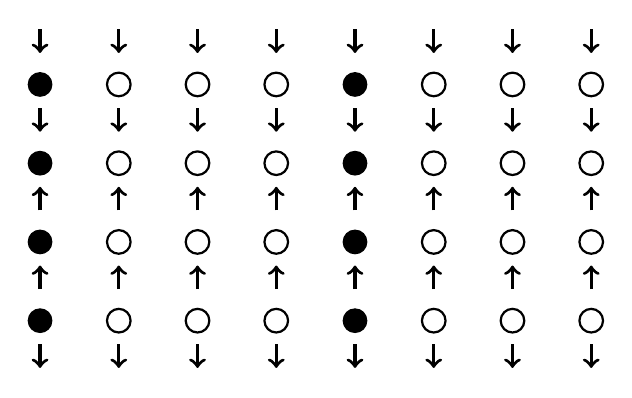
\begin{tikzpicture}
    % charge stripe
    \foreach \y in {0,1,2,3} {
        \foreach \x in {0,4} {
            \filldraw (\x+0,\y) circle [radius=0.15];
            % afm
            \draw [thick] (\x+1,\y) circle [radius=0.15];
            \draw [thick] (\x+2,\y) circle [radius=0.15];
            \draw [thick] (\x+3,\y) circle [radius=0.15];
        }
    }
    
    \foreach \x in {0,1,2,3,4,5,6,7} {
        \draw [very thick, <-] (\x,-0.6) -- (\x,-0.3);
        \draw [very thick, ->] (\x,-0.6+1) -- (\x,-0.3+1);
        \draw [very thick, ->] (\x,-0.6+2) -- (\x,-0.3+2);
        \draw [very thick, <-] (\x,-0.6+3) -- (\x,-0.3+3);
        \draw [very thick, <-] (\x,-0.6+4) -- (\x,-0.3+4);
    }
\end{tikzpicture}
%     \caption[2D phonon anomaly sketch]{Possible 2D real-space scenarios of a coupling between the Cu-O bond-stretching phonon at $q=(0.25,0.25,0)$ and stripe order. Here, the phonon wavector is perpendicular to the stripe direction (parallel to the stripe propagation vector). Small arrows represent displacement of oxygen atoms. Charge oscillations are phason modes of the stripes and the black bars represent charge domain walls. The Lower figure refers to a situation where static charge order lowers the energy of the phonon (intuitively through the change of spring constant). open circles represent hole-poor anti-ferromagnetic Cu atoms and filled circles represent hole-doped ($\frac{1}{2}$ hole per site) Cu atoms.}
%     \label{fig:anomaly_2d}
% \end{figure}

Figure \ref{fig:anomaly_1d} shows a sketch of possible scenarios involving a chain of Cu atoms (circles) separated by oxygen atoms with a certain displacement pattern (arrows). In one scenario \cite{Kaneshita2002}, the charge stripes are fluctuating and the phonon `resonates' with this fluctuation, essentially lowering its energy. In the second scenario \cite{Reznik2006}, static charge order changes the forces between certain Cu-O pairs, an effect that is also minimized at $\bm{Q}_\text{co}$ as shown in the figure. A third possibility is one where the phonon anomaly is found in the perpendicular direction to the one shown in figure \ref{fig:anomaly_1d}. In this case the phonon would resonate with the modulation `within' the charge stripe. Since the softening happens close to $\bm{Q}_\text{co}$ it seems more likely that one of the first two cases are responsible, but it has technically not been settled.

\section{Experiment}
We measured the phonon dispersion highlighted in figure \ref{fig:phonon_anomaly_simulation_summary} in two oxygenated samples: \LCOO{} and \LSCOOsix{} at the triple-axis spectrometer IN8 at ILL. Measuring this phonon dispersion turned out to be more difficult than anticipated, and several attempts were spent in order to reach optimal conditions where we could actually observe the phonon dispersion with relative success.

After our initial attempts, we realized that our signal was contaminated by so-called spurious scattering. While not immediately apparent to us, we identified this `spurion' as accidental Bragg scattering from the analyzer \cite{Shirane2002}. This means that we are in the unfortunate situations where the analyser is at angle where the sample scatters strongly from a structural Bragg peak. While the `job' of the analyser is to select a desired final energy, Bragg scattering is so strong that the signal at the detector will be contaminated by incoherent, scattering from the analyser crystals.

\begin{figure}
    \centering
    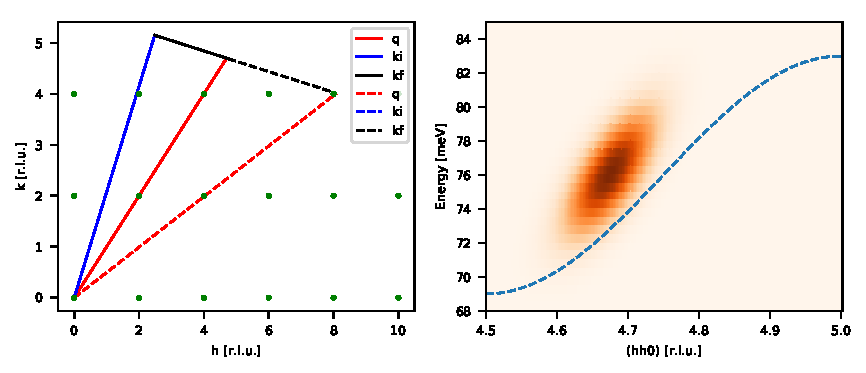
\includegraphics[width=\textwidth]{fig/anomaly/spurion.pdf}
    \caption{\textbf{Left}: Scattering triangle responsible for the A-type spurious scattering (broken lines) at $\bm{Q} = (4.7,4.7,0)$. Green points represent Bragg peaks in the ($h$,$k$)-plane. The (8,4,0) Bragg refection is responsible for the spurious scattering. \textbf{Right}: Simulated effect of the (8,4,0) reflection on a $Q$-$\hbar\omega$ map assuming a Gaussian spurious signal depending on distances in $Q$. Broken line represents a `normal' sinosoidal dispersion in this region as described in the text.}
    \label{fig:in8_spurion}
\end{figure}

Figure \ref{fig:in8_spurion} shows the geometry of this accidental Bragg scattering in reciprocal space. From this sketch we see that the spurious scattering comes from the (8,4,0) reflection. In order to quantify where we would observe this scattering in our measurements, we can make as simulation where we evaluate the strength of the spurion at the desired values of $(\bm{Q}, \omega)$. This is done by constructing the geometry as in \ref{fig:in8_spurion} (top) and then defining the spurious strength through the distance to (8,4,0). The result of such as simulation is shown in figure \ref{fig:in8_spurion} (bottom), and we clearly see that this signal intersects the expected phonon dispersion.

\begin{figure}
    \centering
    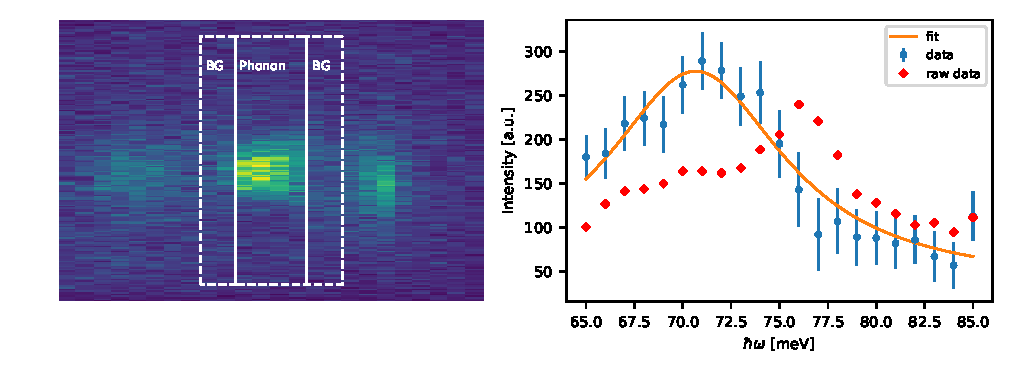
\includegraphics[width=\textwidth]{fig/anomaly/data_reduction.pdf}
    \caption{Illustration of the data reduction performed using the PSD. \textbf{Left}: Summed raw data from an energy scan at $\bm{Q}=(4.65,4.65,0)$. The dashed lines denote the regions of interest (ROI) used in the data reduction. The geometry of the instrument ensures that the desired phonon scattering will occur in the `Phonon' ROI. \textbf{Right}: Corresponding raw (diamonds) and reduced/normalized (circles) data. The raw data is obtained by only considering the `Phonon' ROI, while the reduced data is obtained by subtracting the intensity from the two `BG' ROIs. The solid line is a fit to a DHO lineshape as described in the text.}
    \label{fig:psd_data_reduction}
\end{figure}

Two measures were taken to avoid this spurious scattering. First, by using the goniometers installed on IN8 we can effectively rotate the sample around the [110] axis, which has no affect on our measurements in the [hh0] direction, but does move further away from the condition for spurious scattering since (8,4,0) will be out of the scattering plane. Second, we installed a position-sensitive detector (PSD) with the hope that the spurious scattering is spatially separated from the phonon scattering. It turns out that the spurious scattering indeed can be separated from the phonon as shown in Figure \ref{fig:psd_data_reduction}. Unfortunately, this background subtraction procedure is associated with a large increase in error bars as shown in the figure.

\begin{figure}
    \centering
    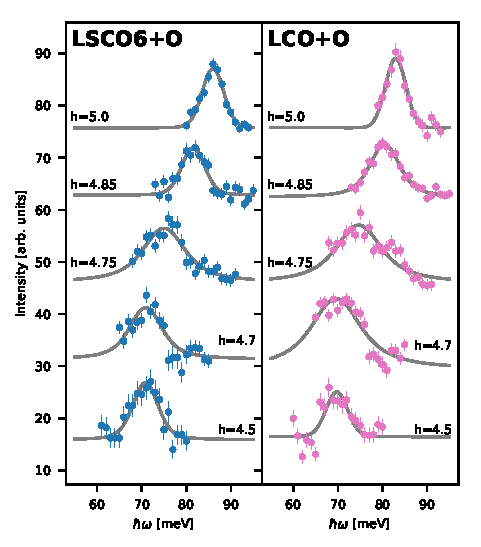
\includegraphics[width=0.49\textwidth]{fig/anomaly/fig2.pdf}
    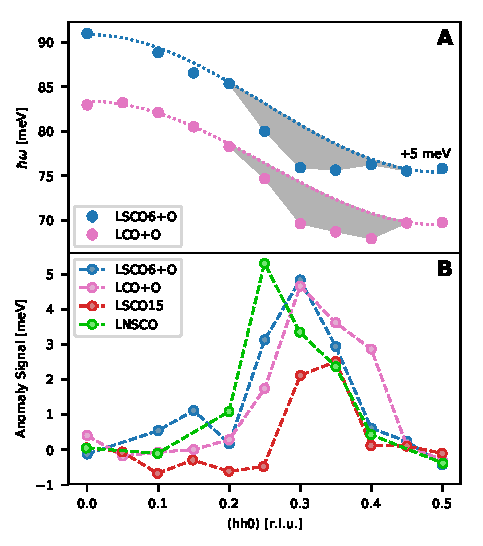
\includegraphics[width=0.49\textwidth]{fig/anomaly/fig3.pdf}
    \caption[Phonon anomaly data and dispersion]{\textbf{Left:} Reduced data at selected wavevectors of the form $Q=(h,h,0)$ for both LSCO6+O and LCO+O at $T=5\,\text{K}$. Data at $\bm{Q}=(5,5,0)$ and $\bm{Q}=(4.85,4.85,0)$ was scaled by a factor of $\frac{1}{2}$ for clarity due to an increase of intensity from the phonon form factor. Data at different $h$ are offset for clarity. Solid lines are fits to a DHO lineshape (see text). \textbf{Right:} \textbf{(A)} Dispersion of the LO phonon obtained from the peak positions of individual spectra of both LCO+O and LSCO6+O (offset by $5\,\text{meV}$ for clarity). Error bars smaller than the markers are not shown. Dashed line is the normal sinusoidal dispersion as described in the text. All data was obtained at $T= 5 \, \text{K}$. \textbf{(B)}: Difference between sinusoidal and measured dispersion in \LCOO{} (LCO+O) \LSCOO{} (LSCO+O), \LSCOopt{} (LSCO15) and \LNSCO{} (LNSCO). Data for LSCO15 and LNSCO adapted from \cite{Reznik2007}.}
    \label{fig:anomaly_data_dispersion}
\end{figure}

Using these procedures, we were able to measure the phonon as shown in figure \ref{fig:anomaly_data_dispersion} for both \LCOO{} (LCO+O)and \LSCOOsix{} (LSCO6+O). The raw data is fit to a Damped Harmonic Oscillator (DHO) model \cite{Fak1997}, which has a Lorentzian shape:

\begin{equation}
    S(\bm{q},\omega) = I_\text{ph} \frac{1}{\pi \omega_{\bm{q}}} \frac{\gamma}{(\omega - \omega_{\bm{q}})^2 + \gamma^2} + I_\text{BG} \, ,
\end{equation}

\noindent where $I_\text{ph}$ is the phonon intensity, $\omega_{\bm{q}}$ the phonon energy at wave vector $\bm{q}$, $\gamma$ the phonon linewidth and $I_\text{BG}$ the background intensity. The extracted dispersion from the data is shown in Fig. \ref{fig:anomaly_data_dispersion} along with a normal sinusoidal dispersion, $\hbar\omega_q=\alpha \cos(2 \pi q) + \beta$, inferred from phonon calculations on LSCO using Density Functional Theory as shown in figure \ref{fig:phonon_anomaly_simulation_summary}. We fit the cosine-function to points near the zone center ($\bm{Q}=(0,0,0))$ and edge $(\bm{Q}=(\frac{1}{2},\frac{1}{2},0))$ to obtain the dashed curves of Fig. \ref{fig:anomaly_data_dispersion}A. To quantify the magnitude of the anomaly, we define the `anomaly signal' as the difference between the normal dispersion and the measured data (gray shaded area in Fig. \ref{fig:anomaly_data_dispersion}A). Fig. \ref{fig:anomaly_data_dispersion}B shows our anomaly signal for \LCOO{} and \LSCOOsix{} along with previous results from optimally doped \LSCOopt{} and insulating, stripe-ordered \LNSCO{} \cite{Reznik2007}. We emphasize the presence of similar anomaly signals on an absolute scale across all studied samples.

\section{Phonon Anomaly and Magnetic Stripe Order}
Since we have now confirmed the presence of a Cu-O bond stretching phonon anomaly in both \LCOO{} and \LSCOOsix{}, we wanted to see if this phonon dispersion could be modified by magnetic fields. The background for this idea is the fact that magnetic stripe order in \LSCO{} has a significant response to magnetic fields in a wide range of doping \cite{Chang2008,Kofu2009,Romer2013,Tranquada2004,Lake2001}. In general, the application of a magnetic field appears to `fill in' the gap of the magnetic excitation spectrum for $x \geq \frac{1}{8}$. While this, in general, is consistent with a picture where the gap is directly related to the superconducting gap, there is evidence that the filled states have a different origin \cite{Kofu2009}. Since one could write books about the spin excitation spectrum in \LSCO{}, I will keep the discussion somewhat limited and refer to the review by \citeauthor{Tranquada2013} \cite{Tranquada2013}.

\begin{figure}[]
    \centering
    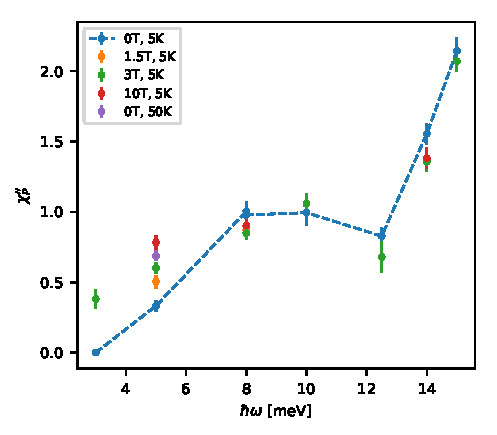
\includegraphics[width=0.5\textwidth]{fig/anomaly/chi.pdf}
    \caption{Amplitude of the magnetic excitation spectrum in \LSCOOsix{} at a variety of fields and temperatures as a function of energy transfer.}
    \label{fig:lscoo_chi}
\end{figure}

Returning to the objective at hand, our idea was to both measure the spin excitation spectrum and anomalous phonons in the same experimental conditions in order to directly probe any correlation (or lack thereof) between the two phenomena. These measurements were only performed for the \LSCOOsix{} sample. Figure \ref{fig:lscoo_chi}A shows the amplitude of the magnetic fluctuations as a function of energy transfer and figure \ref{fig:lscoo_chi}B shows an example of the neutron scattering data used to extract this amplitude. The figure clearly shows that \LSCOOsix{} has gapped excitations which are filled in with the application of a magnetic field. This is in contrast to other oxygen-doped samples (e.g. \LCOO{} \cite{Jacobsen2018}) where the excitations are not gapped.

\begin{figure}
    \centering
    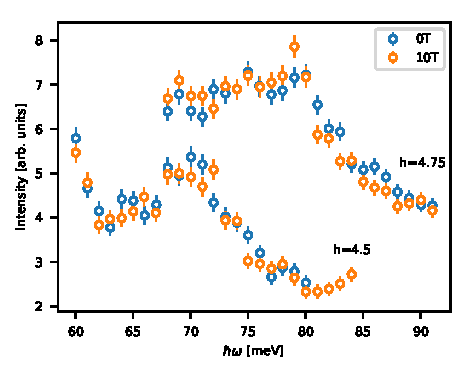
\includegraphics[width=0.5\textwidth]{fig/anomaly/fig4.pdf}
    \caption{Comparison of representative constant-Q ($h$,$h$,0) scans of \LSCOOsix{} in zero-field and with an applied field of $10\,\text{T}$. All measurements performed at $T=5\,\text{K}$}
    \label{fig:in8_lscoo_field}
\end{figure}

In figure \ref{fig:in8_lscoo_field} we have measured the phonon at a `normal' and anomalous wavevector at $T=\SI{5}{\kelvin}$ with and without an applied field of \SI{10}{\tesla}. From this measurement it is thus clear that a field of \SI{10}{\tesla} has no effect on the bond stretching phonon at anomalous wave vectors. 

\section{Discussion}
To begin the discussion of our results, we remark that softening and/or broadening of phonon modes is generally a signature of an incipient structural or electronic instability. Typical examples include structural phase transitions, $\bm{Q}$-dependence of the electron-phonon matrix element, Fermi surface nesting and electronic correlations \cite{Reznik2012}. In order to determine the origin of a given phonon anomaly, it is therefore important to carefully exhaust alternatives before making statements about the connection to novel phases such as dynamic charge stripes \cite{Reznik2012}.

The phonon anomaly appears in vicinity of the wave vector $\bm{Q}_\text{co}=(\frac{1}{4},\frac{1}{4},0)$, consistent with charge stripe ordering as illustrated in Fig. \ref{fig:anomaly_1d}. Measurements of LNSCO \cite{Reznik2008b}, LSCO15 \cite{Reznik2007} and LBCO \cite{Reznik2007} have shown a suppression of the anomaly as one moves away from the bond-stretching direction \cite{Reznik2008b}, supporting a one-dimensional stripe-like picture. Additionally, the phonon anomaly in LSCO15 and LBCO has almost no temperature dependence apart from a slightly sharper peak shape when heating from $10\,\text{K}$ to $300\,\text{K}$ \cite{Reznik2006,Reznik2007}. These phenomena rule out anharmonicity and structural inhomogeneity as mechanisms for the phonon anomaly in these systems.

A combination of inelastic X-ray and ARPES measurements on overdoped LSCO ($x=0.2$ and $x=0.3$) have shown that the phonon anomaly wavevector is inconsistent with Fermi surface nesting \cite{Park2013,Park2014}, contradicting the idea of a phonon softening due to a Kohn anomaly. A different, possibly $\bm{Q}$-dependent, electron-phonon coupling could still be responsible for the phonon anomaly. Such an effect would renormalize the electronic quasiparticle dispersion (the so-called `ARPES kink' \cite{Garcia2010}) at energies similar to the phonon softening. The ARPES kink has been observed in LSCO $x=0.2$ and $x=0.3$, but since only LSCO $x=0.2$ shows anomalous phonons, the two phenomena appear to not be connected \cite{Park2014}.

Thus, all previous studies are unable to explain the phonon anomaly through conventional means and any coupling to stripe order is likely dynamic. One possible scenario is a coupling of the Cu-O bond-stretching phonon with steeply dispersing charge fluctuations. \citeauthor{Kaneshita2002} performed calculations based on the Hubbard model of this scenario, predicting anomalous phonon dispersions due to both transverse (meandering) and longitudinal (compression) coherent stripe fluctuations \cite{Kaneshita2002} (see Fig. \ref{fig:anomaly_1d} for a sketch of the transverse mode). We emphasize that the observed phonon anomaly reported here (see Fig. \ref{fig:anomaly_data_dispersion}) and in LBCO/LSCO \cite{Reznik2006, Reznik2007} is remarkably similar to the calculation by \citeauthor{Kaneshita2002} (see Fig. 5 in \cite{Kaneshita2002}).

Despite differences in the magnetic excitation spectra as recorded by neutron scattering (including low and zero energy transfers), the three materials LCO+O, LSCO6+O and LSCO15 have remarkably similar in-plane Cu-O bond-stretching dispersions (Fig. \ref{fig:dispersion}). Furthermore, static charge order at zero field has been observed in a different sample of LCO+O \cite{Zhang2018} and in LNSCO \cite{Tranquada1996} but so far not in LSCO6+O nor in LSCO15. These observations together rule out a unique, direct connection between static stripes (spin and charge) and the phonon anomaly. In order to further confirm this point, we performed scans of LSCO6+O at selected wave vectors in a $H=10\,\text{T}$ magnetic field which is known to induce a considerable volume of stripe-like magnetic order in this particular sample \cite{Holm2019}. While static charge order has not been observed in LSCO6+O, measurements on LSCO ($x=0.12$) have shown that static charge and spin stripes respond identically to magnetic fields \cite{Christensen2014}.

Figure \ref{fig:in8_lscoo_field} contains data at two wave vectors with and without an applied magnetic field of $10\,\text{T}$, clearly showing the absence of any detectable field effect on the in-plane Cu-O bond-stretching phonon at $\bm{Q}=(\frac{1}{4},\frac{1}{4},0)$. These measurements were performed simultaneously with measurements of the low-energy magnetic fluctuations as shown in figure \ref{fig:lscoo_chi}, confirming a significant increase in the magnetic spectral weight towards lower energies consistent with the appearance of field-induced stripe-order \cite{Holm2019}. Thus, the appearance of static magnetic stripe order does not affect the phonon anomaly in LSCO6+O. A similar insensitivity of the phonon anomaly to an applied magnetic field has been observed in underdoped ($T_\text{c} = 66\,\text{K}$) YBa$_2$CuO$_{6.6}$ \cite{Reznik2016}.

We have shown that the phonon anomaly is a robust feature in optimally doped  as well as stripe-ordered cuprates which is independent of the structural details related to the doping process. Since it is equally well-formed in stripe-ordered and optimally doped systems, where the latter show no static magnetic order, the anomaly is surprisingly insensitive to low-energy magnetic characteristics. This is further confirmed by the absence of a magnetic field effect in LSCO6+O which introduces static magnetic stripe-order.

The phonon anomaly is strongest in the doping region around optimal $T_\text{c}$ ($0.125 \le n_\text{h} \le 0.20$) (LSCO15, LNSCO \cite{Reznik2007}, LBCO \cite{Reznik2006}, LSCO6+O, LCO+O), regardless of the presence of static charge order (LNSCO \cite{Tranquada1995}, LBCO \cite{Fujita2004}), suppression of bulk superconductivity (LNSCO \cite{Tranquada1996}) or dopant disorder (LCO+O, LSCO6+O). In addition, the phonon anomaly is unaffected by magnetic fields (LSCO6+O, YBa$_2$CuO$_{6.6}$ \cite{Reznik2016}) and temperature (LBCO, LSCO15) \cite{Reznik2007}). Thus it appears to be an intrinsic, robust signature of doped cuprates near optimal doping.

If fluctuating stripes are the fundamental degrees of freedom relevant for the cuprates, it is appealing to draw a connection to Pair-Density-Wave superconductors \cite{Fradkin2015}. In this system, the fundamental degrees of freedom are transverse charge fluctuations in an `electronic liquid crystal' phase without long range order \cite{Kivelson1998}. In this scenario, the phonon anomaly in materials without static stripe order is due to a matching of the phonon wavevector with, otherwise undetectable, short-range transverse stripe correlations. The $x=\frac{1}{8}$ anomaly then corresponds to the special case where stripes exhibit long-range order. 

In conclusion, we have measured the in-plane Cu-O bond-stretching phonon in LSCO6+O and LCO+O and provided evidence for significant anomalous behavior. Since one sample (LCO+O) exhibits charge order \cite{Zhang2018} while the other (LSCO6+O) does not \cite{Holm2019}, and since the samples also have different magnetic spectra with distinct field dependencies \cite{Jacobsen2018, Holm2019} we conclude that the phonon anomaly has no direct, trivial relationship to either magnetic or charge static order. In addition, the unique structural characteristics of oxygen-doped samples rule out a connection between the specific dopant species and the phonon anomaly. We proceed to conclude that the phonon anomaly is a signature of transverse charge stripe fluctuations, which is a common characteristic of the cuprate family and appears to be a pre-requisite to optimal superconductivity in these systems.

\section{Summary}
in this chapter we performed measurements of anomalies in a specific high energy mode possibly related to stripe order. In contrast to previous chapters, we can finally connect a feature in the phonon dynamics to superconductivity-related concepts. This is possibly due to the fact that the other measurements were less focused on specific modes and more the overall shape. Also in contrast to the previous chapters, there seems to be no difference between the anomalies discovered here and in samples with other dopants.

% \section{Origin of the phonon anomaly}
% Phonon anomalies in materials can, in general, happen for a number of reasons. The Cu-O bond-stretching phonon anomaly in LSCO does not seem to be caused by any of the conventional phenomena, and a relationship to novel charge modes has been proposed. One such charge mode is fluctuations of stripe order. The appeal of this interpretation is the near impossibility of measuring dynamic charge stripes directly. The phonon anomaly could thus provide an indirect way of investigating the elusive properties of dynamic charge stripes. Given the hypothesis that the phonon anomaly and dynamic charge stripes are related, what are then the possible mechanisms of the coupling? A couple of scenarios are given in Figure \ref{fig:anomaly_2d} and \ref{fig:anomaly_1d}.

% The charge oscilation was introduced by \citeauthor{Kaneshita2002}\cite{Kaneshita2002} in a theoretical study of stripes coupling to the phonon. The Kohn anomaly picture was introduced in context of LBCO by \citeauthor{Reznik2006}\cite{Reznik2006} as an intuitive way to explain the connection between the phonon and stripe wavevectors. The 2D picture in Figure \ref{fig:anomaly_2d} has only been mentioned (to my knowledge) by \citeauthor{Reznik2010} in his two reviews on the phonon anomaly\cite{Reznik2010, Reznik2012}. Note, it appears that the Kohn anomaly picture has been ruled out by ARPES measurements by \citeauthor{Park2014}\cite{Park2014}


% \begin{figure}
%     \centering
%     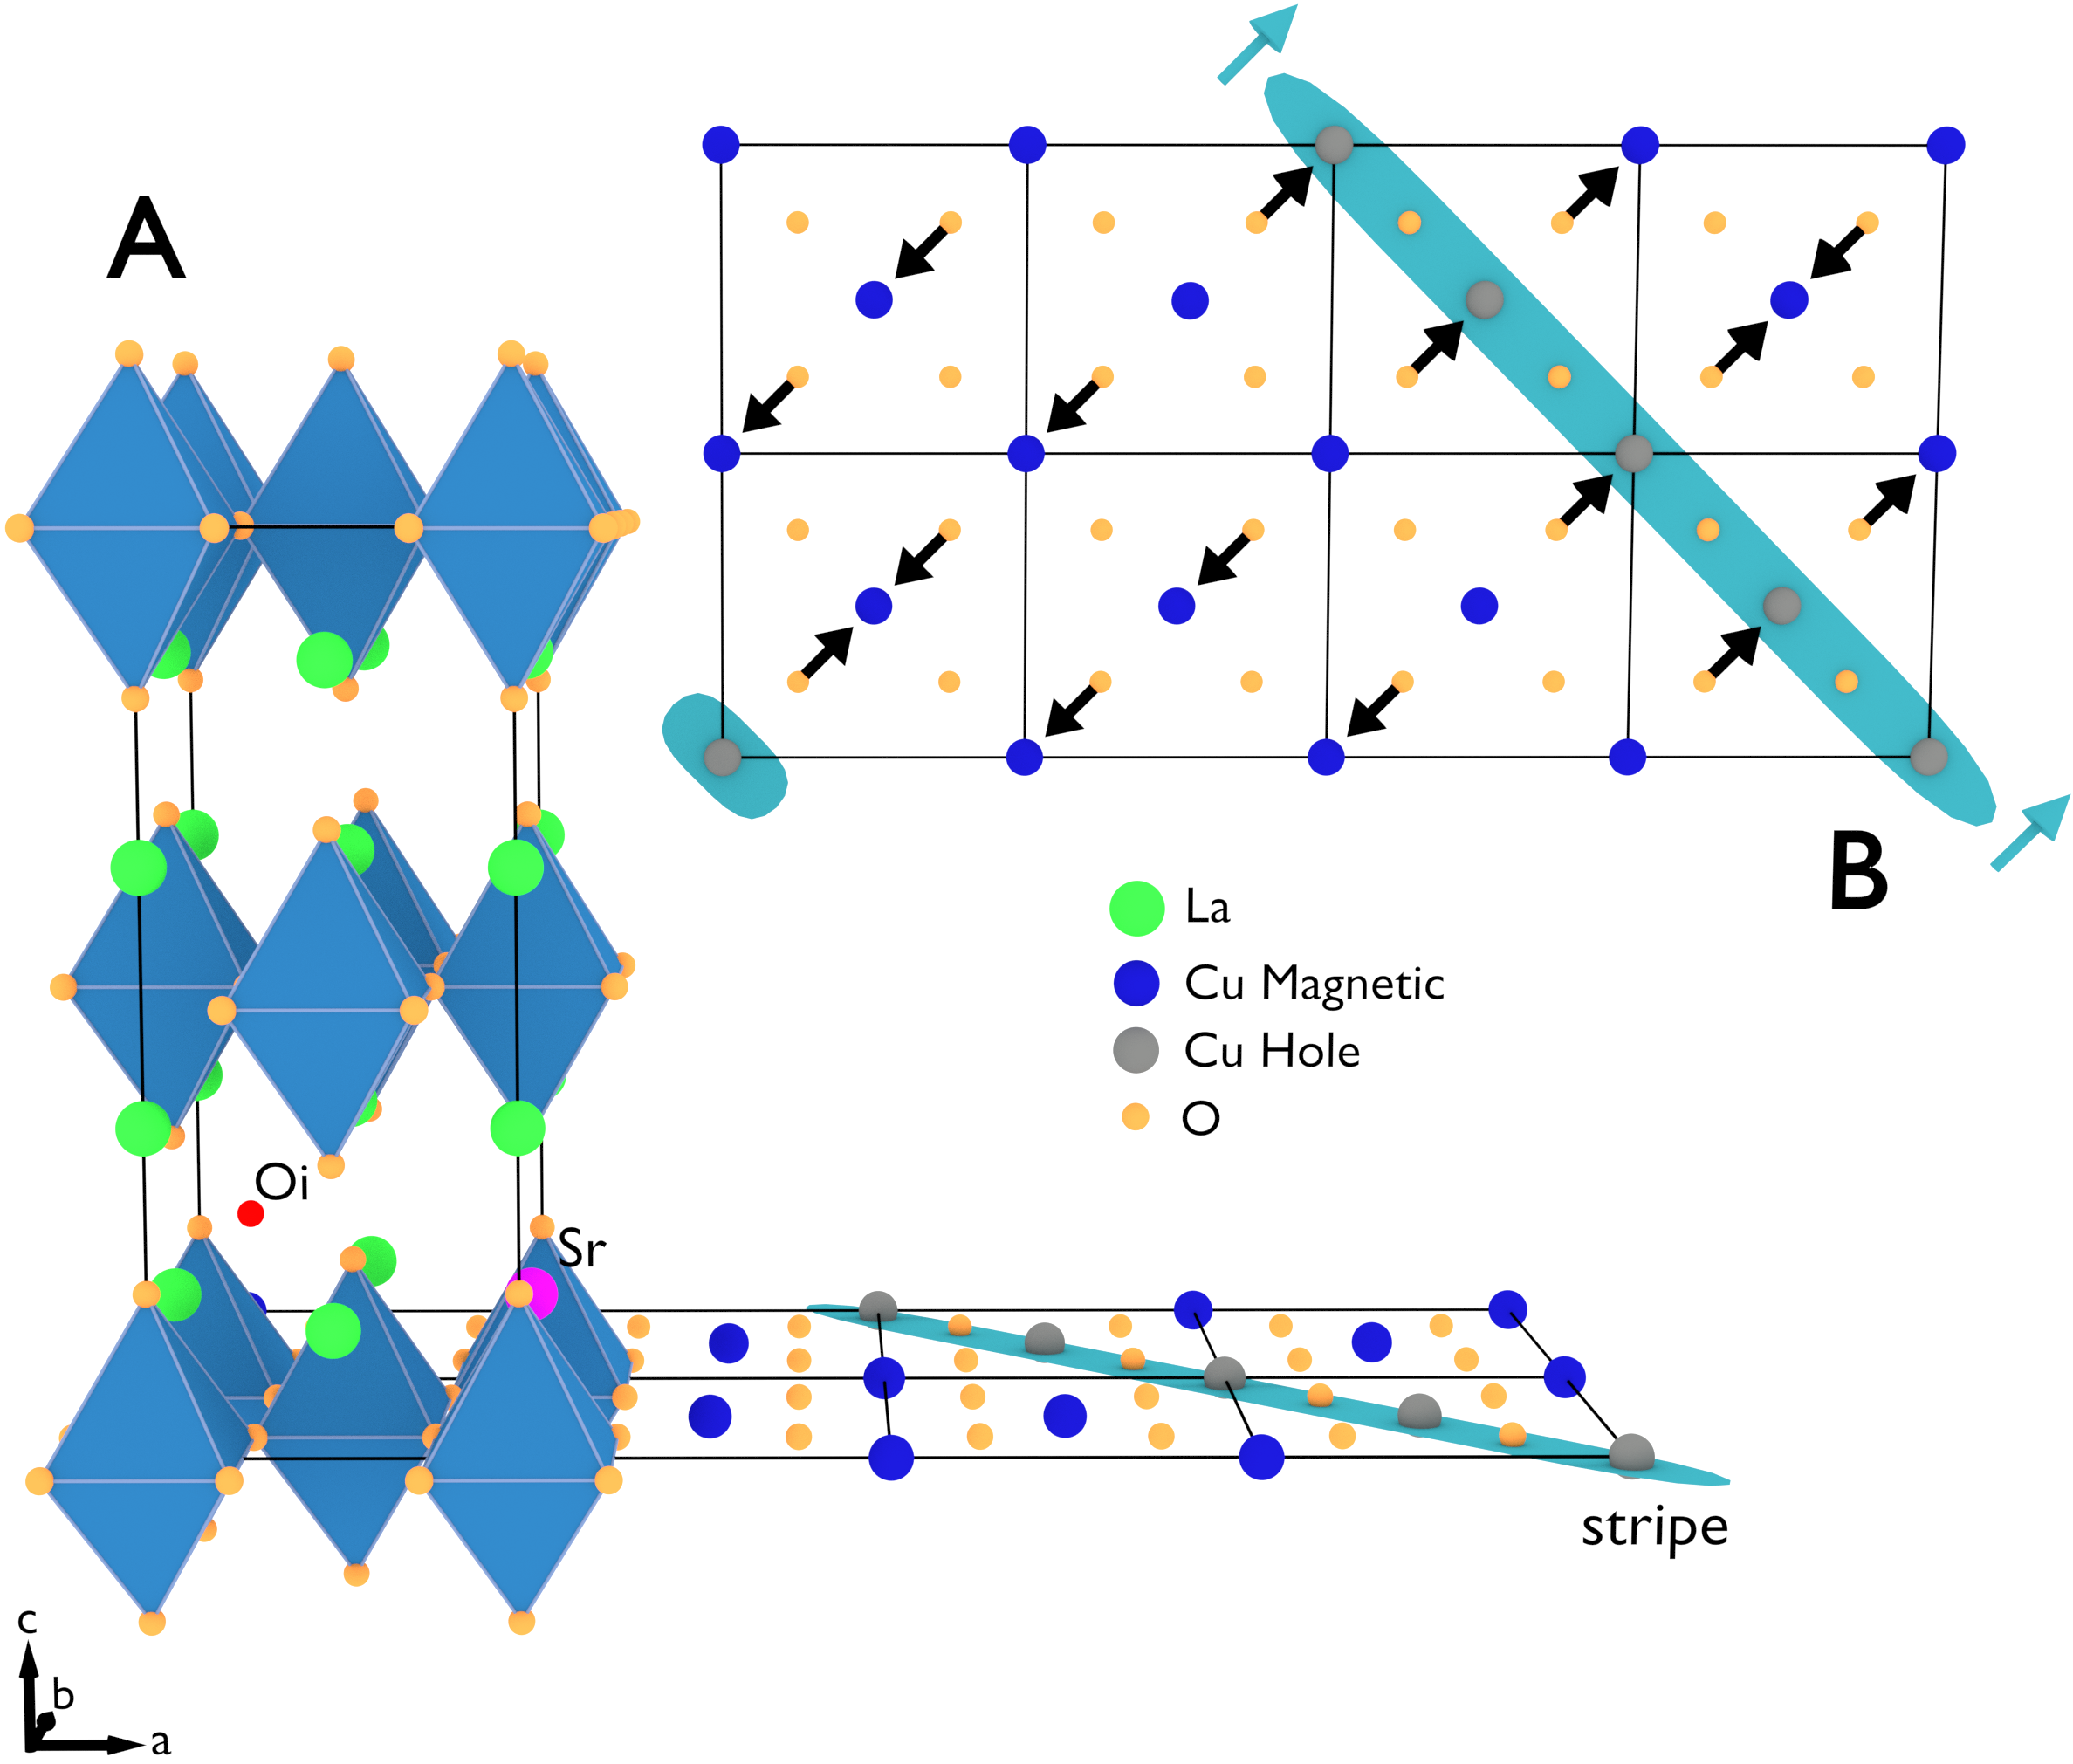
\includegraphics[width=0.7\textwidth]{fig/anomaly/fig1.png}
%     \caption[Crystal structure annotated with phonon at (0.25,0.25,0) and stripe order]{Sketch of crystal LSCO+O crystal structure containing two distinct dopants in a $4 \times 2 \times 1$ orthorhombic unit cell. The two singular Sr/O dopants correspond to a hole doping of $n_h = \frac{3}{32} \approx 0.09$. Dark blue are magnetic Cu sites while light blue represents hole-rich Cu sites. This period-4/8 segregation into charge/magnetic regions is known as stripe formation \cite{Tranquada1995}. Inset: Possible matching of stripe dynamics with the Cu-O bond stretching mode at q=$(0.25,0.25,0)$ as proposed by \citeauthor{Kaneshita2002} \cite{Kaneshita2002}.}
%     \label{fig:crystal_anomaly}
% \end{figure}

% \begin{figure}
%     \centering
%     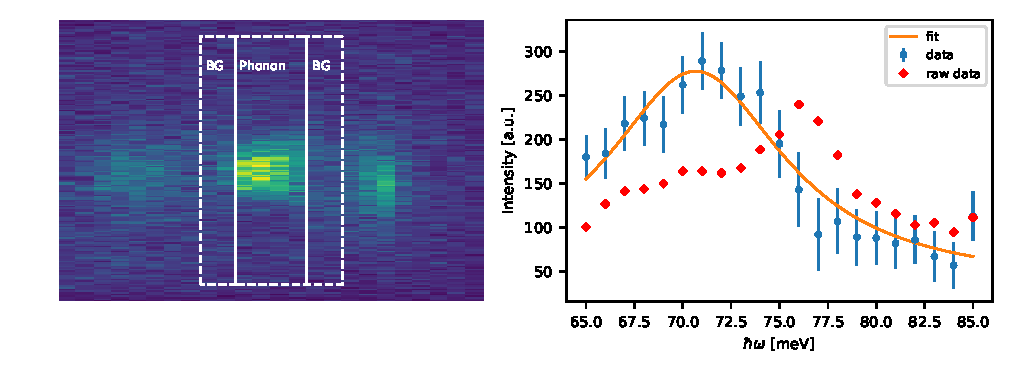
\includegraphics[width=0.54\textwidth]{fig/anomaly/data_reduction.pdf}
%     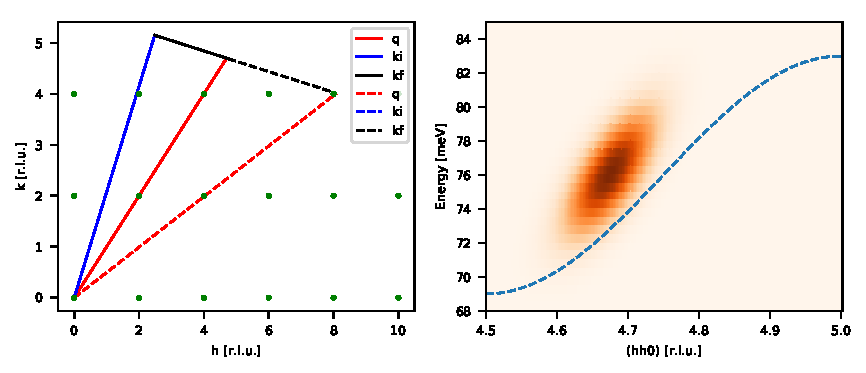
\includegraphics[width=0.45\textwidth]{fig/anomaly/spurion.pdf}
%     \caption[IMPS data reduction and Spurion vizualisation]{\textbf{Top-left:} Raw data (summed from one constant-$Q$ scan) from the IMPS 2D detector. The phonon signal is observed in the central area and spurious signal is seen towards the edges. Broken white lines mark the areas used for data reduction. \textbf{Bottom-left:} Result of data reduction using the defined areas. We are clearly able to separate the phonon and spurious signal with this procedure. \textbf{Top-Right:} Scattering triangle responsible for the A-type spurious scattering (broken lines) at $Q=(4.7,4.7,0)$. The culprit is the (8,4,0) reflection. \textbf{Bottom-right:} Simulated effect of the (8,4,0) reflection on a $Q$-$\hbar\omega$ map assuming a Gaussian spurious signal depending on distances in $Q$. Broken line represents a `normal' (not anomalous) dispersion in this region.}
%     \label{fig:imps_data_reduction}
% \end{figure}



% \begin{figure}
%     \centering
%     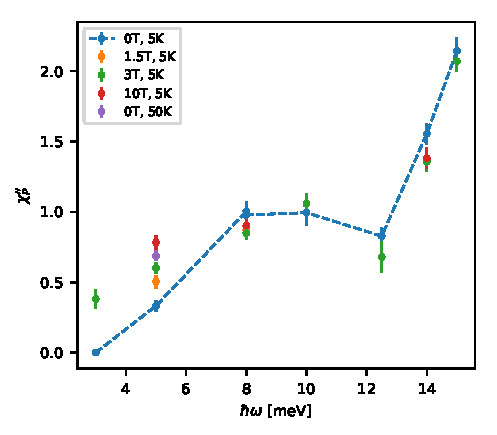
\includegraphics[width=0.49\textwidth]{fig/anomaly/chi.pdf}
%     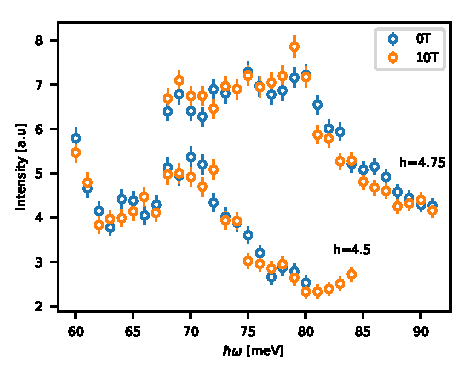
\includegraphics[width=0.49\textwidth]{fig/anomaly/field_selected.pdf}
%     \caption[LSCO6+O magnetic field effect on fluctuations and phonon]{\textbf{Left:} Imaginary part of the magnetic susceptibility in LSCO6+O as a function of energy transfer, field and temperature. As shown, a field of \SI{3}{\tesla} is sufficient to open a gap in the magnetic excitation spectrum. \textbf{Right:} Raw phonon data at anomalous ($h=4.75$) and normal $h=4.5$ wave vectors as a function of field. Contrary to the magnetic excitation spectrum, the anomalous phonon does not appear to be modified by an applied field.}
%     \label{fig:phonon_chi_field}
% \end{figure}

% \section{Things deleted from paper}

% \subsection{PDW Stuff in detail}
% As is usual with the cuprates, it is difficult to find a framework that captures all of the experimental evidence. With that in mind, we relate our findings to the concept of intertwined orders, while keeping in mind that oxygen-doped samples are macroscopically phase seperated. Intertwined orders are described with reference to pair-density-wave (PDW) superconductivity as the parent microscopic order from which $d$-wave superconductivity, magnetic order, charge order and others emerge\cite{Fradkin2015}. The PDW formalism predicts simultaneous ordering temperatures, gapless magnetic excitations\cite{Christensen2016} and an `electronic liquid crystal' phase\cite{Kivelson1998} that emerges from transverse fluctuations in the charge-density-waves (CDW) of neighbouring stripes. These fluctuations then become the fundamental degrees of freedom relevant to superconductivity. This is consistent with the fact that we see the phonon anomaly whenever the CDW is present, regardless of the nature of the transverse fluctuations. This could potentially explain the `sharper' phonon anomaly in static stripe-ordered LNSCO (Figure DISPERSION)

% %Note that I have never seen Reznik or Tranquada imply this connection, so it might be a bit too speculative?

% Returning to LCO+O, LSCO6+O and LSCO15, this would explain the discrepancy in magnetic signatures while still having similar $T_\text{c}$ and phonon anomaly, if we assume that the magnetic domains between the fluctuating stripes can be tuned separately\todo{not sure if this is the case, but in the original papers, electronic liquid phase is described without considering magnetism}. In the case of static charge order and magnetism, this is not the case\cite{Christensen2014}. Another scenario is one in as sample without separate domains of static and fluctuating stripes in which the magnetic field only modifies spectral weight at low energies while not affecting the phonon mode at $\approx 80\,\text{meV}$. A measurement of the phonon anomaly in field of static stripe ordered LSCO ($x=0.12$) would help resolve these issues. A significant disceprency in this interpretation is that fact that LSCO+O is macroscopically phase separated, so the question remains if the two phases are entirely segregated or if exactly one of them contains the physics described here\todo{Linda can you weigh in?}.

% \subsection{Chemical disorder - not sure if relevant}
% It has been suggested that the inhomogeneous charge distribution due to dopant ions can cause a renormalization of elementary excitations\cite{Park2011}. By adding optimally superconducting, oxygen-doped samples to the list of samples with strong phonon anomalies, we rule out any connection between the phonon anomaly and specific dopant disorder.

% \subsection{Discussion}
% The results of our measurements (Figure DISPERSION) clearly show the similarity of anomalous behavior between optimally doped LSCO15 and oxygen-overstoichiometric L(S)CO+O. Due to the difference in dopant species, we believe that an immediate result of these measurements is a confirmation of the relationship between fluctuating charge order in the CuO$_2$ planes and the giant phonon anomaly as proposed by \citeauthor{Reznik2012}\cite{Reznik2012}. In the following discussion, we work under the hypothesis that fluctuating charge order in LSCO15 and L(S)CO+O is expressed in the same way despite the different chemistries and bulk characteristics of the two compounds. We start by reviewing some important results from LSCO literature.

% It is well established that stripe order is ubiquitous in the cuprates, but a correlation with superconductivity remains elusive and maintaining an internal consistency between measurements is challenging. Neutron scattering, $\mu$SR, NQR and NMR experiments of $T_m$ have shown that static magnetic stripes in LSCO appear at $x=0.03$, take a maximum at $x=0.125$ (where $T_\text{c} \approx 25$ has a minimum) before disappearing abruptly\cite{Julien2003, Hirota2001}. In contrast dynamic magnetic stripes have been observed throughout the superconducting dome, with a gap opening in the spin excitation spectrum for $0.125 < x < 0.20$\cite{Kofu2009, Lee2000, Gilardi2004}. On the other hand, samples considered in this letter both exhibit static magnetic stripes\todo{REF?}, have a gap of 3 meV (LSCO+O)\todo{REF?} and no gap (LCO+O)\cite{Wells1997, Jacobsen2018}, while sharing an optimal $T_\text{c} \approx 40\,\text{K}$. With these results in mind, it is natural to question a trivial relationship between static and dynamic magnetic stripes. Recent measurements by \citeauthor{Jacobsen2018} on LCO+O show a discrepancy in the momentum-transfer of static and dynamic magnetic stripes\cite{Jacobsen2018}, directly showing that the perceived connection might be coincidental.

% If the magnetic signal from stripes occur with a modulation of $\delta_\text{m}$, the charge component appears with a modulation of $\delta_\text{c} = 2\delta_\text{m}$. In LSCO static charge stripes have been found for a narrow range of doping ($0.12 < x < 0.13$)\cite{Thampy2014, Croft2014} at the expected position with $\delta_\text{c} = 0.25$. In addition, the static magnetic and static charge stripes have an identical response to magnetic field in LSCO ($x=0.12$) below $T_\text{c}$, indicating a strong connection between the two phenomena\cite{Christensen2014}. Dynamic charge order has, to our knowledge, never been directly observed in LSCO.

% Despite the experimental inconsistencies outlined above, we believe that unifying observations of stripe order would be a significant step in our quest to understand superconductivity in the cuprates. The nature of dynamic charge order is a significant missing piece in the stripe picture. The `giant' phonon anomaly observed in LBCO, LSCO, YBCO and now L(S)CO+O represents significant progress in finding said piece. While phonon anomalies, in general, can happen for a number of reasons, the connection to stripe order comes in multiple flavours\cite{Reznik2012}. First, the phonon anomaly obeys the symmetry of charge stripes appearing at $\delta_\text{c} \approx 0.25$. The 1D nature of the phonon anomaly is verified from experiments showing a disappearance of the phonon anomaly by deviating slightly from the Cu-O bond direction\todo{REF?}. ARPES and Inelastic X-ray Scattering (IXS) experiments on LSCO ($x=0.20$)\cite{Park2014} have shown that the phonon anomaly cannot be caused by Fermi Surface nesting (Kohn anomaly). Theoretically, it has been proposed that the phonon anomaly can be explained as steeply dispersing charge fluctuations intersecting the optical phonon branch\cite{Kaneshita2002}

% Perhaps the most appealing feature of the phonon anomaly is the apparent correlation with $T_\text{c}$. In LSCO ($x=0.20$ and $x=0.15$), the anomaly amplitude is larger than for samples outside or on the edge of the superconducting dome. The samples studied in this letter follow this trend by having slightly larger $T_\text{c}$ and anomaly amplitudes compared to their LSCO15 cousin.

% With this in mind, we believe that the results contained in Figure \ref{fig:dispersion} proves the hypothesis of \citeauthor{Reznik2012} \cite{Reznik2012} that the phonon anomaly is connected to charge fluctuations in the CuO$_2$-planes. Our samples are chemically distinct to LSCO15 and each other, but exhibit identical behavior in terms of the energy scale of the phonon dispersion and the anomaly amplitude. The lack of field effect in Figure FIELD is surprising, but consistent with results on YBCO\todo{REF?}. On the other hand, the phonon anomaly has almost no temperature dependance, indicating that the fluctuations are extremely robust.

% \subsection{Old stuff 1}
% In addition, the magnitude of this gap $E_g$ has been suspected to track $T_\text{c}$ through the relation $T_c = 1.5 E_\text{g}/k_\text{B}$\cite{Kofu2009}. The samples considered in this letter contradicts this suspicion by having comparable $T_\text{c} \approx 40\,\text{K}$, while LCO+O exhibits no gap\cite{Jacobsen2018,Wells1997} while LSCO+O has a gap of $E_g \approx 3.5$ meV, similar to LSCO15\cite{Lee2000}.


% The controversy is rooted in the fact that static stripe order appears to suppress superconductivity while their fluctuations have been proposed to promote superconductivity. It thus becomes natural to ask if the static and dynamic stripe order arises from the same electronic phenomenon and if they are separate phases that can be tuned individually. 

% In either case, stripe order has manifestations of competing orders. A notorious example is the `$T_\text{c}$ anomaly' in LSCO, where a suppression of $T_c$ happens at $n_h=\frac{1}{8}$ along with measurable static magnetic and charge order\cite{Christensen2014,Croft2014,Thampy2014}, which is not present in optimally doped LSCO15. In non-superconducting, tetragonal LNSCO and LBCO, similar features have been observed\cite{Wilkins2011}. In addition, \citeauthor{Christensen2014} have shown, by performing experiments in magnetic fields, that the static charge and spin order is connected\cite{Christensen2014}.

% Fluctuating magnetic order has been extensively studied throughout the LSCO phase diagram, revealing a connection between 1) the incommensurate modulation $\delta$ of the antiferromagnetic parent phase and 2) the hole doping $n_h$. $\delta$ is equal to $n_h$ up to a saturation at $\delta = n_h = \frac{1}{8}$[yamada], once again stressing the ubiquity of this `$\frac{1}{8}$ phase' in the cuprates.

% A playground for understanding this `zoo' of orders is the LSCO+O system, which separates\cite{Mohottala2006} into distinct magnetic ($n_h=\frac{1}{8}$) and superconducting phases\cite{Udby2013}. In addition, the mobile nature of the dopants severely reduces flux pinning\cite{Mohottala2008}, indicating that annealed disorder allows the superconducting part of the sample to emerge in a cleaner way.

% From the $T_c$ anomaly in LSCO, phase separation in LSCO+O, the incommensurability $\delta$ of magnetic fluctuations and the insulating nature of LNSCO and LBCO12, we believe that the `$\frac{1}{8}$ phase' is a necessary, but not sufficient precursor for superconductivity. The question then remains: How are the magnetic and charge fluctuations related to this phase and how are they expressed in experiments?

% An appealing picture that unite these features is one of simultaneous structural and electronic phase separation in real space, with 1) the $\frac{1}{8}$ non-superconducting phase  expressed by static order and 2) the superconducting phase containing fluctuating charge and magnetic order. Due to the quenched disorder of LSCO this separation only becomes apparent around $n_h = \frac{1}{8}$, while the annealed disorder in LSCO+O results in detectable phase separation at optimal doping.

% While subtle, several experiments support this picture. \citeauthor{Kofu2009} reports a different origin of spin fluctuations in LSCO around the $\frac{1}{8}$ anomaly ($x=0.125,0.13.0.135$) above and below a spin gap at $\approx 4$ meV through detailed measurements of the intrinsic linewidth of the excitations. Recently \citeauthor{Jacobsen2018}\cite{Jacobsen2018} reported a different origin in momentum space of the static and dynamic spin stripes through high-resolution measurements of the incommensurability $\delta$ in LCO+O (The same sample studied in this letter). 

% Real-space structural phase separation in LCO+O has been probed by X-ray micro-diffraction. \citeauthor{Poccia2012} showed a spatial anti-correlation between two kinds of oxygen orderings\cite{Poccia2012} and in the single-layered cuprate HBCOO ($T_c = 95\,\text{K}$) containing oxygen interstitials, \citeauthor{Campi2015} found a nano-scale spatial anti-correlation between Oxygen-rich and CDW-rich regions\cite{Campi2015}.

% We hypothesize that novel charge fluctuations contain vital elements of the pairing mechanism in cuprates, but that SC only arises when the stripe phase is realized locally. In this picture charge fluctuations survive above $T_c$, but SC is realized only as we approach static stripe order.

% Starting from our assumption that the phonon anomaly is an expression of steeply dispersing charge fluctuations intersecting an optical phonon branch\cite{Kaneshita2002}, the above picture explains the difference between LSCO15, LNSCO and L(S)CO+O. LNSCO is close to superconductivity, but the specific local structure induced by the addition of Nd$^3+$ ions prevents the `good' charge fluctuations to separate from the $\frac{1}{8}$ phase. The stronger local energetics due to structure produces a steeper dispersion, resulting in a strongly peaked anomaly at $h=\frac{1}{4}$ (charge component of $\frac{1}{8}$ phase). LSCO15 and L(S)CO+O, on the other hand, have an optimal local structure allowing superconductivity to emerge unscathed. The slightly better superconducting properties of the oxygen-overstoichiometric samples are thus reflected in the broader and stronger anomalies. This is also consistent with the experiments performed by \citeauthor{Park2014}\cite{Park2014}, where the strength of the anomaly is found to scale with $T_c$.

% Finally, even though we are able to populate the $\frac{1}{8}$ phase with a magnetic field in LSCO+O (Udby et al, to be published) the charge fluctuations connected to SC are completely untouched by a field of 10T ($\ll H_{c2}$) and this is reflected in the absence of modifications of the anomaly (See Figure FIELD).
